\chapter{Optimizing the Neural Network Model}
{\color{red}LZ: this chapter can be removed}
\section{General Training Procedure}
We have discussed the Gradient-based back propagation procedure for vanilla neural networks. In this chapter we will discuss in detail various optimization techniques. Let's start with summarizing the basic procedure of training a neural network model.

The key elements of training a neural network model can be summarized as follows: 
\begin{enumerate}
\item Model construction: choose hyper-parameters, activation function, loss function.
\item Obtain a training data set and a test data set.
\item Adjust the parameters with an optimization methods such as gradient descent to reduce the value of the loss function over the training set. The gradient of the loss function is back propagated through each layer.
\item Apply the model to the test set to check for overfitting or underfitting.
\item Repeat the training and testing step until the model is well-trained.
\end{enumerate}





\section{Other Optimization Methods}


Stochastic Gradient Descent (SGD) is currently the favourite optimization method in deep learning. Its popularity is gained thanks to its ease of implementation and the nonconvexity of the optimization problem.

Despite its popularity and its low cost per step, SGD has well-known 
deficiencies that can make it inefficient, or at least tedious to use in 
practice. Two main issues are that 1) SGD requires a step size (learning 
rate) that has drastic effect on the algorithm's efficiency, is often 
difficult to choose well, and virtually never optimal for each individual 
descent step; 2) SGD is inherently sequential: it is very difficult to 
parallelize them using GPUs or distribute them using computer clusters.

Batch methods, such as Limited memory BFGS (L-BFGS) or Conjugate Gradient 
(CG), with the presence of a line search procedure, are usually much more 
stable to train and easier to check for convergence. These methods also 
enjoy parallelism by computing the gradient on GPUs and/or distributing that 
computation across machines. These methods, conventionally considered to be 
slow, can be fast thanks to the availability of large amounts of RAMs, 
multicore CPUs, GPUs and computer clusters with fast network hardware.

A weakness of batch L-BFGS and CG, which require the computation of the 
gradient on the entire dataset to make an update, is that they do not scale 
gracefully with the number of examples.

\subsection{Learning with Momentum}
The momentum technique is a compromise that can smooth out the erratic behaviour caused by a fixed learning rate in SGD without slowing down the learning process too much. The idea is to update the weights with the moving average of the individual weight changes corresponding to single training patterns.
If we label everything by the time $t$, then implementing a moving average can be computed as:

\begin{equation}
\label{emom}
\aligned
\Delta \bm W_k(t+1) :=& \bm{W_k}(t+1) - \bm{W_k}(t) = r\frac{\partial L_{total}}{\partial \bm{W_k}}(\bm{W_1}(t),...,\bm{W_d}(t),\bm{\theta_1}(t),..,\bm{\theta_d}(t)) -  \eta\Delta\bm W_k(t)\\
\Delta \bm \theta_k(t+1) :=& \bm{\theta_k}(t+1)-\bm{\theta_k}(t) = r\frac{\partial L_{total}}{\partial \bm{\theta_k}}(\bm{W_1}(t),...,\bm{W_d}(t),\bm{\theta_1}(t),..,\bm{\theta_d}(t)) - \eta\Delta \bm\theta_k(t)
\endaligned
\end{equation}
Here we introduce a new hyper-parameter $\eta$ and a momentum term $\eta\Delta
\bm W_k(t)$ or $\eta\Delta\bm \theta_k(t)$. The momentum simply adds a fraction of the previous update to the current one.  When the gradient keeps pointing in the same direction, this will increase the size of the steps taken towards the minimum. If $\eta=0$, then it is the same as the gradient descent algorithm used before. When using the momentum method, it is usually necessary to reduce the learning rate $r$ accordingly so that the learning step is not too large.



\subsection{Gradient Descent with Line Search}

In neural network model we are seeking parameter values such that the loss function 
$$L_{total}(\bm{W_1},...,\bm{W_d},\bm{\theta_1},..,\bm{\theta_d})$$
is minimal. One idea is to consider this as a one-dimensional optimization problem that optimizes one parameter while holding the other parameters fixed. We can do this for each parameter, and repeat the process until all weights are simultaneously at optimal values.

Another idea about training neural network is to find the optimal learning rate with line search. Instead of a fixed learning rate, let's consider it as another variable $r$. Let $\bm{W_1}(t)$,...,$\bm{W_d}(t)$, $\bm{\theta_1}(t)$,..., $\bm{\theta_1}(t)$ be the value of weight matrices and bias vectors at time $t$. By the update rule \eqref{ebpup}, the updated value for these parameters are
\begin{equation}
\aligned
\bm{W_k}(t+1) =& \bm{W_k}(t) - r_k\frac{\partial L_{total}}{\partial \bm{W_k}}(\bm{W_1}(t),...,\bm{W_d}(t),\bm{\theta_1}(t),..,\bm{\theta_d}(t))\\
\bm{\theta_k}(t+1) =& \bm{\theta_k}(t) - r_k'\frac{\partial L_{total}}{\partial \bm{\theta_k}}(\bm{W_1}(t),...,\bm{W_d}(t),\bm{\theta_1}(t),..,\bm{\theta_d}(t))
\endaligned
\end{equation}

The loss function can be treated as a function of one variable 
$$
L_{total} = L_{total}(r_k) = L_{total}(\bm{W_k}(t) - r_k\frac{\partial L_{total}}{\partial \bm{W_k}}).
$$ 
Its derivative can be computed as
\begin{equation}
L_{total}'(r_k) =\frac{\partial L_{total}}{\partial \bm{W_k}}(\bm W_k(t+1))\circ \frac{\partial L_{total}}{\partial \bm{W_k}}(\bm W_k(t)).
\end{equation}

Treat the gradient $\frac{\partial L_{total}}{\partial \bm{W_k}}$ as a vector. If $L_{total}'(r_k) =0$, the direction of the new update $\frac{\partial L_{total}}{\partial \bm{W_k}}(\bm W_k(t+1))$ should be orthogonal to the previous update $\frac{\partial L_{total}}{\partial \bm{W_k}}(\bm W_k(t))$. Together with one-dimensional optimal search such as the Golden section method and the Brent's method, one can find a small interval for $r$ such that the value corresponding to the minimum of the loss function lies in the interval. Note that during this process multiply forward passes are needed, as the target function needs to be evaluated at several different points. Also for each weight matrix and each bias vector, an optimal learning rate needs to be computed separately. If we want to find a global optimal learning rate that applies to all parameters, we will need to consider to following equation:

\begin{equation}
\aligned
&L'(r)\\ =& \sum_{k=1}^d \big(\frac{\partial L}{\partial \bm{W_k}}\frac{\partial \bm{W_k}}{\partial r} + \frac{\partial L}{\partial \bm{\theta_k}}\frac{\partial \bm{\theta_k}}{\partial r}\big)\\
=& -\sum_{k=1}^d\big(\frac{\partial L}{\partial \bm{W_k}}(\bm{W_1}(t+1),...,\bm{W_d}(t+1),\bm{\theta_1}(t+1),..,\bm{\theta_d}(t+1))\frac{\partial L_{total}}{\partial \bm{W_k}}(\bm{W_1}(t),...,\bm{W_d}(t),\bm{\theta_1}(t),..,\bm{\theta_d}(t))\\
 &+ \frac{\partial L}{\partial \bm{\theta_k}}(\bm{W_1}(t+1),...,\bm{W_d}(t+1),\bm{\theta_1}(t+1),..,\bm{\theta_d}(t+1))\frac{\partial L_{total}}{\partial \bm{\theta_k}}(\bm{W_1}(t),...,\bm{W_d}(t),\bm{\theta_1}(t),..,\bm{\theta_d}(t))\big)
\endaligned
\end{equation}

In this case the derivative is a polynomial in $r$ of degree $d$. Solving such equation is going to be more costly. Therefore in general gradient descent with line search is not faster than the basic gradient descent method.

 
%----------------------------------------------------------------------------
\subsection{Limited Memory BFGS Method}

Besides first-order optimization methods, one can use second-order methods which seek the place where the gradient vanishes. We will start with the classical Newton's method:
\begin{equation}
\bm{z} \leftarrow \bm{z} - \big[HL(\bm{z})\big]^{-1}\nabla L(\bm{z}).
\end{equation}
Here, $\bm{z}$ is a vector representing all parameters of a neural network model, $HL(\bm{z})$ is the Hessian matrix, which is a square matrix of second-order partial derivatives of the function, and $\nabla L(\bm{z})$ is the gradient vector. More precisely, $\bm{z}$, $HL(\bm{z})$, and $\nabla L(\bm{z})$ are defined as follows:
\begin{equation}
\aligned
\bm{w_j} :=& ((\textit{1st column of }\bm{W_j})^T, (\textit{2nd column of }\bm{W_j})^T,..., (\textit{last column of }\bm{W_j})^T), j=1,...,d\\
\bm{z} :=& (\bm{w_1}^T,..., \bm{w_d}^T, \bm{\theta_1}^T,...,\bm{\theta_d}^T)^T = (z_1,...,z_N)\\
h_{ij} =& \frac{\partial^2 L}{\partial z_i \partial z_j}, i,j=1,...,N\\
HL(\bm{z}) =& \big(h_{ij}\big)_{i,j=1}^N\\
\nabla L(\bm{z}) =& (\frac{\partial L}{\partial z_1},...,\frac{\partial L}{\partial z_N})
\endaligned
\end{equation}

Intuitively, the Hessian matrix describes the local curvature of the loss function, which allows us to perform a more efficient update. In particular, multiplying by the inverse Hessian matrix leads the optimization to take more aggressive steps in directions of shallow curvature and shorter steps in directions of steep curvature. However, the update above is impractical if the depth of the neural network model is large, since it requires the inversion of the entire Hessian matrix corresponding to parameters from each layer. In this section we will introduce a \textit{quasi-Newton} method called the Broyden-Fletcher-Goldfarb-Shanno (BFGS) algorithm that seek to approximate the inverse of the Hessian matrix. 

The derivation starts with the quadratic model
\begin{equation}
m_k(\bm{p}) = f(\bm{x_k}) + \nabla f(\bm{x_k})\bm{p} + \frac{1}{2}\bm{p}^TB_k\bm{p},
\end{equation}
where $B_k$ is a symmetric positive definite matrix that will be updated in every iteration.

Given this convex quadratic model, we can write down the minimizer $\bm{p_k}$ explicitly as
\begin{equation}
\bm{p_k}=-B_k^{-1}\nabla f(\bm{x_k}).
\end{equation}

The key difference compared with the classical Newton's method is that we are using an approximate Hessian $B_k$ that can be obtained by updating the previous $B_{k-1}$ with only a few arithmetic operations. We impose the following condition on each update: $m_{k+1}(\bm{p})$ must match the gradient of the objective function in $\bm{x_k}$ and $\bm{x_{k+1}}$. Thus we have
\begin{equation}
\aligned
B_k(\bm{p_k}) =& -\nabla f(\bm{x_k})\\
B_{k+1}(\bm{p_{k+1}}) =& -\nabla f(\bm{x_{k+1}})\\
B_{k+1}(\bm{x_{k+1}} - \bm{x_k}) =& \nabla f(\bm{x_{k+1}}) - \nabla f(\bm{x_k})\\
%\nabla m_{k+1}(-\alpha_k\bm{p_k})=&\nabla f(\bm{x_{k+1}}) - \alpha_k B_{k+1}\bm{p_k} = \nabla f(\bm{x_k})
\endaligned
\end{equation}


%We derive that
% \begin{equation}
% \label{ebk}
% \alpha_k B_{k+1} \bm{p_k} = \nabla f(\bm{x_{k+1}}) - \nabla f(\bm{x_k})
% \end{equation}

%We clean up the notations by introducing
\begin{equation}
\aligned
\bm{s_k} :=& \bm{x_{k+1}} - \bm{x_{k}}\\
\bm{y_k} :=& \nabla f(\bm{x_{k+1}}) - \nabla f(\bm{x_{}})\\
\endaligned
\end{equation}

Now the condition on $B_{k+1}$ can be expressed as
\begin{equation}\label{esecant}
\bm{B_{k+1}s_k} = \bm{y_k}.
\end{equation}
There are infinitely many symmetrical matrices that satisfy equation \eqref{esecant}. The BFGS method seeks the one that requires fewest changes upon $\bm B_k$, i.e., the solution to the following problem:
\begin{equation}
\aligned
\min_{\bm{B_{k+1}}}&\|B_{k+1} - B_k\|\\
s.t.&\bm{B_{k+1}s_k} = \bm{y_k}\\
&\bm{B_{k+1}^T} = \bm {B_{k+1}}
\endaligned
\end{equation}
Here we use the \textit{weighted Frobenous norm} {(\color{red}definition needed)}. The optimal solution is given by
\begin{equation}
\label{ebfgs}
\bm{B_{k+1}} = \big(I - \rho_k\bm{y_ks_k^T}\big)\bm{B_k}\big(I - \rho_k\bm{y_ks_k^T}\big)+\rho_k\bm{s_ks_k^T},
\end{equation}
where $\rho_k = (\bm{y_ks_k^T})^{-1}.${\color{red}(proof?)}

{\bf Limited-memory BFGS method.} By equation \eqref{ebfgs}, each $\bm{B_k}$ can be obtained recursively from $(\bm{s_k, y_k})$, $(\bm{s_{k-1}, y_{k-1}})$,...,$(\bm{s_1, y_1})$. This would require the algorithm to maintain a history of all these vectors, which could be a huge burden. The Limited-memory BFGS (L-BFGS) method simply truncates this procedure, using only last $m$ pairs of vectors to construct the matrix $\bm B_k$. This results in a loss of accuracy in approximation, but it will greatly reduce the momery requirement of this algorithm.
% In order to ensure that the solution is a local minimum, we will impose the \textit{strong Wolfe condition} on curvature:
% \begin{equation}
% Wolfe condition.
% \end{equation}

% By pre-multiplying equation \eqref{ebk} by $\bm{s_k^T}$ we have
% \begin{equation}
% 0 < \bm{s_k^TB_{k+1}s_k} = \bm{s_k^T y_k}.
% \end{equation}


{\bf Cost and convergence rate.} The cost of the BFGS method per iteration is dominated by matrix-vector multiplication in equation \eqref{ebfgs} ($O(n^2)$). Other computations include function evaluations and gradient evaluations. The convergence rate is super-linear. Newton's method converges quadratically, but the cost per iteration is higher since it requires the solution of a linear system. In addition, Newton's method requires the calculation of second derivatives whereas the BFGS method does not.








\section{Back-Propagation of Convolutional Neural Networks}

In general, the convolution operation is a mathematical operation on two functions (f and g); it produces a third function, that is typically viewed as a modified version of one of the original function.

\begin{itemize}
\item
Convolution
$(f*g)(x) := \int_{-\infty}^{\infty}f(t)g(x-t)dt$
\item
Discrete convolution
$(f*g)[n] := \sum_{-\infty}^\infty f[m]g[n-m]$
\item
2-Dimensional convolution
$(F*G)[i,j] := \sum_{s = -\infty}^\infty\sum_{t = -\infty}^\infty F[s, t]G[i-s, j-t]$
\end{itemize} 

In neural network applications, the input is a multidimensional array (referred to as tensors), and so are the parameters adapted by the algorithm. In CNN terminology, the first function $f(x)$ is referred to as the input, the second function $g(x)$ is referred to as the kernel (or filter), and the output function $(f*g)(x)$ is referred to as the feature map. If we use 2D images $M\in\mathbb{R}^{n\times n}$ as input and use a 2D filter $F\in\mathbb{R}^{d\times d}$ we have
$$(M*F)[i,j] := \sum_{s = 0}^{d-1}\sum_{t=0}^{d-1} F[s, t]G[i+s, j+t], i,j,=0,...,n-d-1$$. Here the output matrix $(M*F)$ is an $(n-d)\times(n-d)$ matrix, and the kernel is flipped comparing to the previous definition. Convolution in CNN is illustrated as in Figure \ref{fconv}
\begin{figure}[ht]
\label{fconv}
\centering
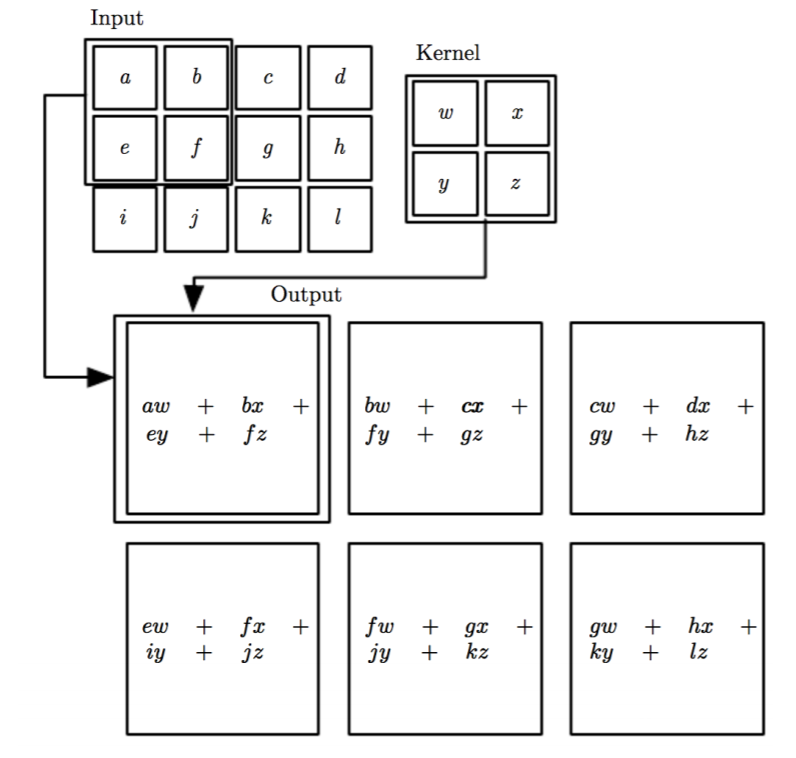
\includegraphics[scale=0.4]{Convolution1.png}
\caption{Convolution in CNN}
\end{figure}
{\bf Convolutional Neural Network (CNN)} is the most widely-used neural network structure for tasks on image pattern recognition. A CNN mainly comprises three types of layers: fully-connected (FC) layers, convolutional layers, and pooling layers
\begin{figure}[ht]
\centering
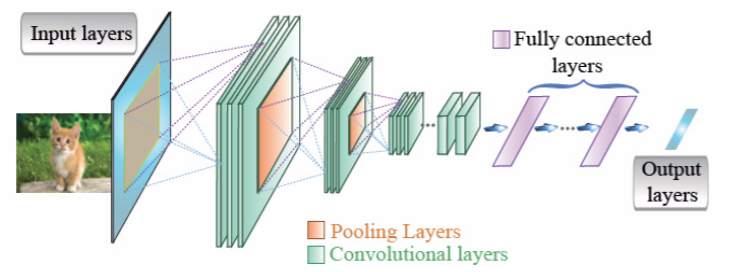
\includegraphics[scale=0.7]{CNN.png}
\caption{Convolutional Neural Network}
\end{figure}

{\bf Structure of CNN}
A convolution layer in CNN is a composition of three functions: $f^{conv}$, $f^{sig}$, and $f^{pool}$

{\bf Convolutional Layer} consists of a set of filters/feature maps $F_{ij} = \big(f_{ijkl}\big)_{k,l}$ (matrices of size $d\times d$ such as $d=3,5$). During the forward pass, each filter will conduct a 2D convolution with the input matrices $X_i=\big(x_{ikl}\big)_{kl}$ across its width and height. In this way local-features can be extracted and fed into subsequent layers to get higher-order features. We use 3-dimensional tensor $\mathcal{X}=\big(x_{ikl}\big)_{i,k,l}$ to represent the set of input matrices, and 4-dimensional tensor $\mathcal{F}=\big(f_{ijkl}\big)_{i,j,k,l}$ to denote the set of filters in a convolutional layer. We have that
%At a convolution layer, the previous layer’s feature maps are convolved with learnable kernels and put through the activation function to form the output feature map. Each output map may combine convolutions with multiple input maps. In general, we have that
\begin{equation}
\aligned
f^{conv}(\mathcal{X}, \mathcal{F}) =& \big(y_{jst}\big)_{j,s,t}=:\mathcal{Y}\\
y_{jst} =& \sum_i\sum_{k,l} x_{i,s+k, t+l}f_{ijkl}\\
f^{sig}(\mathcal{Y}) =& \big(\sigma(y_{jst})\big)_{j,s,t}=:\mathcal{Z}
\endaligned
\end{equation}

{\bf Pooling layer}. Pooling layer subsamples statistics to obtain summary statistics that are invariant to shifts and distortions in some degree. Commonly used pooling functions are
\begin{enumerate}
\item
Mean pooling: $f^{pool}(\mathcal{Z})=\big(\frac{\sum_{k=1}^m z_k}{m}\big)$
\item
Max pooling: $f^{pool}(\mathcal{Z})=\big(\max_{1\le k\le m}\{z_k\}\big)$
\item
$l^p$ pooling: $f^{pool}(\mathcal{Z})=\big(\|(z_1,...,z_m)\|_p\big)$
\end{enumerate}


\begin{figure}[ht]\label{fcnnbp}
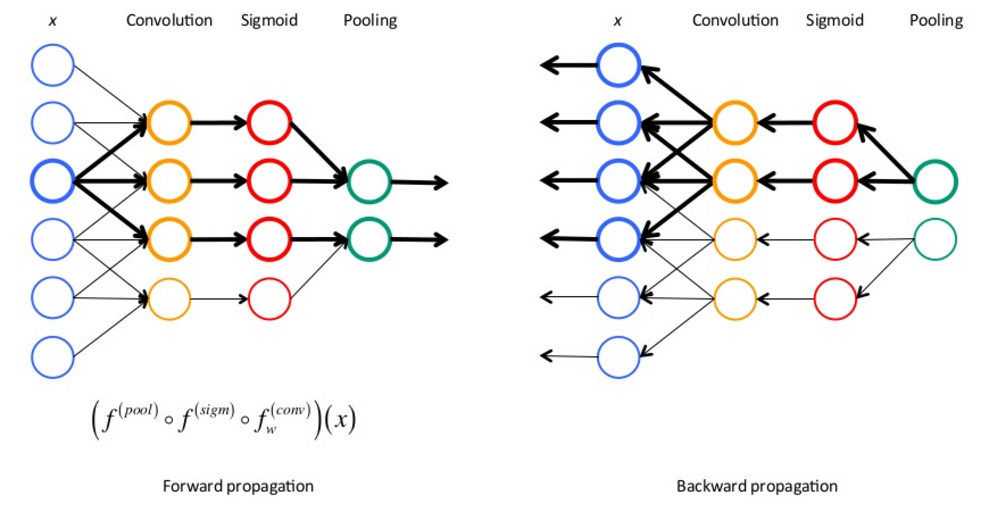
\includegraphics[scale=0.5]{CNNBP}
\caption{Convolutional Layer}
\end{figure}

Figure \ref{ffea} illustrates features extracted the first three convolutional Layers  on a facial recognition task.

\begin{figure}[ht]
\label{ffea}
\centering
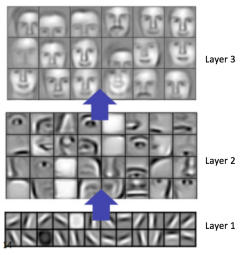
\includegraphics[scale=1]{Features.png}
\caption{Features}
\end{figure}

{\bf Backpropagation in CNN}.
To back-propagate through one convolutional layer, one need to compute the derivative of three functions:
\begin{equation}
\aligned
\bm\delta^{conv}_{ikl} =& \frac{\partial L}{\partial x_{ikl}} =
\sum_{j,k,l}\frac{\partial L}{\partial y_{jkl}}\frac{\partial y_{jkl}}{\partial x_{ikl}} = \sum_{k,l=0}^{r-1}\bm\delta^{sig}_{ikl}\\
\bm\delta^{sig}_{jkl} =& \frac{\partial L}{\partial y_{jkl}} = \sigma'(y_{jkl})\\
\bm\delta^{pool}_{jkl} =& \frac{\partial L}{\partial z_{jkl}} = \frac{\partial L}{\partial x^{next}_{jkl}}\frac{\partial x^{next}_{jkl}}{\partial z_{jkl}} = \bm\delta^{next, conv}_{jkl}\\
\frac{\partial L}{\partial f_{ijkl}} =& \sum_{j,k,l}\frac{\partial L}{\partial y_{jkl}}\frac{\partial y_{jkl}}{\partial f_{ijkl}}=\sum_{s,t=0}^{d-1}\bm\delta^{sig}_{jst}x_{i, s+k, t+l}
\endaligned
\end{equation}
The partial derivative of the pooling function is usually called the \textit{upsample} function. For example. for the max pooling function, the corresponding upscale function is $\mathbbm{1}_{z_{jkl} = \max\{z_k\}}$ (distributing the gradient to the entry with maximum value). Also note that the partial derivative of the filer parameters are computed through a discrete convolution.









\section{Tensor Computation and Decomposition}

{\bf Tensor}
\begin{itemize}
\item
Definition of tensor: an element $\mathcal{F}\in\mathbb{R}^{I_1\times\cdots\times I_N}$.
\item
Element-wise: 
$$
\mathcal{F}[i_1,...,i_N]\in\mathbb{R}, i_j=1,...,I_j, j=1,...,N.
$$
\item
Fiber: mode-1 tensor (vector) obtained by fixing every index but one.
\item
Slice: mode-2 tensor (matrix) obtained by fixing every index but two.
\item
Norm: 
$$
\|\mathcal{F}\| := \sqrt{\sum_{i_1=1}^{I_1}\cdots\sum_{i_N=1}^{I_N} \mathcal{F}[i_1,...,i_N]^2}
$$
\end{itemize}
\begin{figure}[ht]
\centering
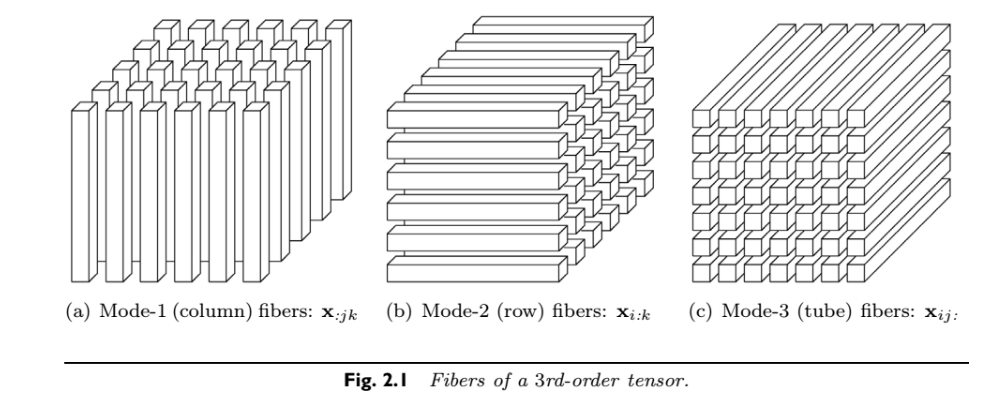
\includegraphics[scale=0.5]{fiber.png}
\end{figure}
\begin{figure}[ht]
\centering
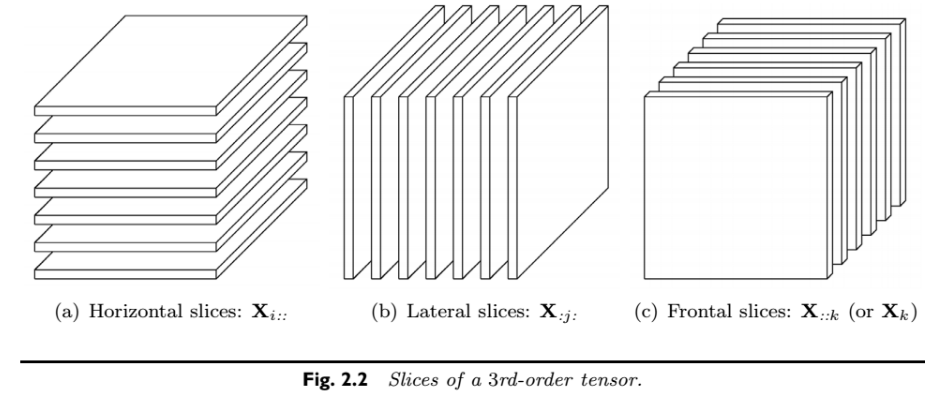
\includegraphics[scale=0.5]{slice.png}
\end{figure}

{\bf Metricization}
The mode-$n$ metricization of a tensor $\mathcal{X}\in\mathbb{R}^{I_1\times\cdots\times I_N}$ is denoted by $X_{(n)}$ and arranges the mode-$n$ fibers to be the columns of the resulting matrix.
\begin{figure}[ht]\label{fmat}
\centering
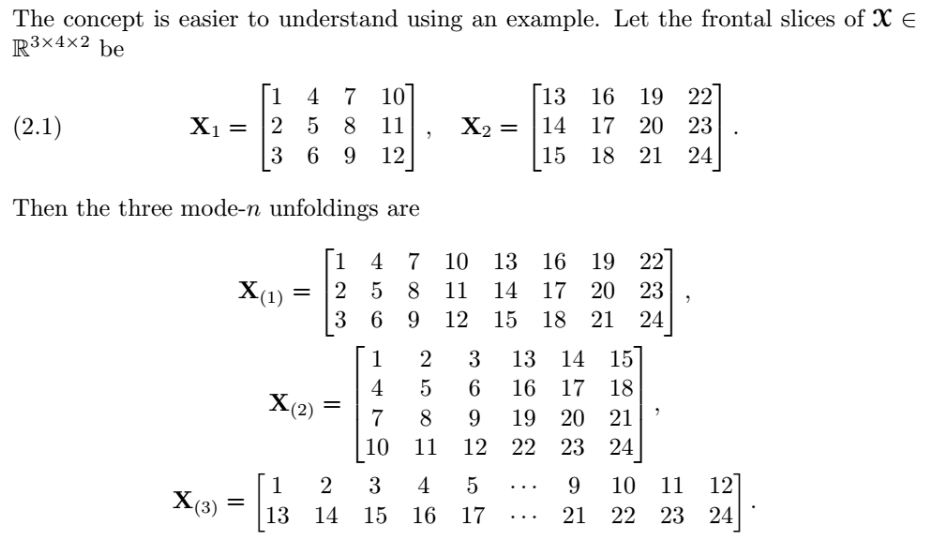
\includegraphics[scale=0.6]{metricization.png}
\caption{Tensor Matricization}
\end{figure}
{\color{red} Definition of Matricization}. An example is given in Figure \ref{fmat}.

{\bf CP Decomposition}
The CANDECOMP/PARAFAC (CP) decomposition attempts to decompose a tensor as a sum of rank-1 tensors:

\begin{equation}
\mathcal{X}[i_1,...,i_N] = \sum_{k=1}^r a^{(1)}_{i_1k}a^{(2)}_{i_2k}\cdots a^{(N)}_{i_Nk}
\end{equation}
The number of summation is call the CP-rank of tensor $\mathcal{X}$.
\begin{figure}[ht]
\centering
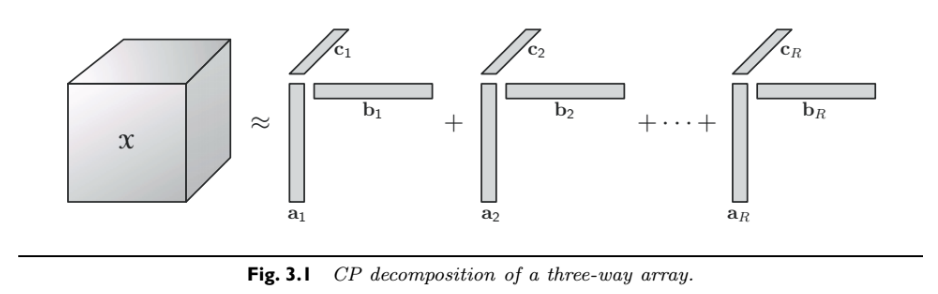
\includegraphics[scale=0.6]{CP_decomposition.png}
\end{figure}

{\bf Challenges about CP Decomposition}
\begin{itemize}
\item
The problem of finding the CP-rank of a tensor is NP-hard.
\item
For a general 3-mode tensor $\mathcal{X}\in\mathbb{R}^{I\times J\times K}$, its maximal attainable rank is bounded by
$$
rank(\mathcal{X})\le \min\{IJ, JK, KI\}
$$
\item
Unlike matrices, the low-rank approximation problem for tensors is not well-defined: \textit{any rank-3 tensor can be infinitely approximated by a rank-2 tensor}.
\end{itemize}

{\bf Tucker Decomposition}

The \textit{Tucker-decomposition} is a form of higher-order PCA. It decomposes a tensor into a core tensor multiplied by a matrix along each mode.
\begin{figure}[ht]
\centering
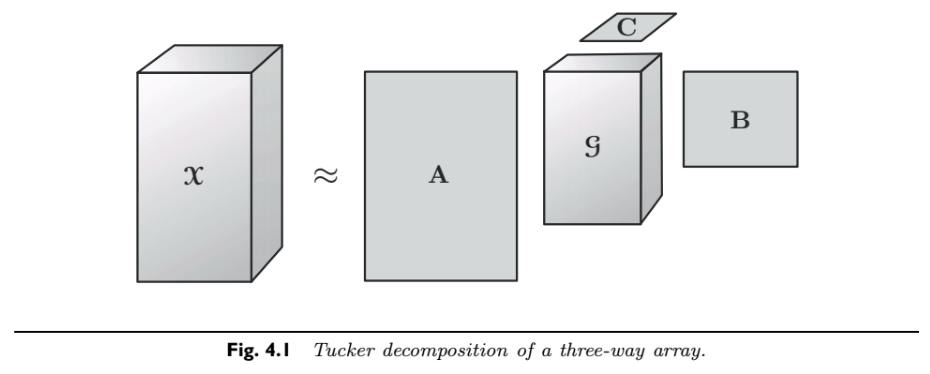
\includegraphics[scale=0.6]{Tucker.png}
\end{figure}
\begin{equation}
\mathcal{X}[i,j,k] = \sum_{p=1}^P\sum_{q=1}^Q\sum_{r=1}^R
g_{pqr}a_{ip}b_{jq}c_{kr}, i=1,...,I, j=1,...,J, k=1,...,K.
\end{equation}

{\bf Tensor-Matrix Multiplication}
Tucker decomposition is best illustrated through \textit{tensor-matrix multiplication}. A product of a tensor $\mathcal{X}$ and a matrix $\bm M=\big(m_{ij}\big)_{i,j}$ on the $k$-th mode is a tensor defined as:
\begin{equation}
    \big(\mathcal{X}\times_kM\big)[i_1,...,i_n] = 
    \sum_j \mathcal{X}[i_1,...,i_{k-1},j,i_{k+1},...,i_n]m_{ji_k}.
\end{equation}
$M\times_k\mathcal{X}$ can be defined similarly as
\begin{equation}
    \big(M\times_k\mathcal{X}\big)[i_1,...,i_n] = 
    \sum_j m_{i_kj}\mathcal{X}[i_1,...,i_{k-1},j,i_{k+1},...,i_n]m_{i_kj}.
\end{equation}
The following properties are easily provable:
\begin{lemma}
[Tensor-Matrix Multiplication]
\begin{equation}
\aligned
&(\mathcal{X}\times_k M)\times_l N = (\mathcal{X}\times_l N)\times_k M =: \mathcal{X}\times_k M\times_l N\\
&(\mathcal{X}\times_k M)\times_k N = \mathcal{X}\times_k(M\cdot N)
\endaligned
\end{equation}
\end{lemma}
{\color{red}proof?}

With the notation above, the Tucker decomposition can be written as
\begin{equation}
\label{etucker}
\mathcal{X} = \bm P\times_1 \bm Q\times_2 \bm R\times_3 \mathcal{G}
\end{equation}
{Tucker Rank}
Tucker rank (P, Q, R) is defined through the matricization:
\begin{align*}
P = rank(\mathcal{X}_{(1)})\\
Q = rank(\mathcal{X}_{(2)})\\
R = rank(\mathcal{X}_{(3)})\\
\end{align*}

As a result, matrix SVD and low-rank approximation can be extended to the computation of Tucker ranks (HOSVD). 

{\bf Tensor-Train Decomposition}
The need for storing the $I_1\times\cdots\times I_n$ core tensor makes the Tucker decomposition increasingly unattractive as $N$ gets larger. The following definition of Tensor Train decomposition solves the problem, while preserving the possibility of SVD-based compression and low-rank approximation:
\begin{definition}
A tensor $\mathcal{X}\in\mathbb{R}^{I_1\times\cdots\times I_n}$ is said to have \textit{tensor train rank (TT)} $(r_1, r_2,...,r_{N-1}, r_N)$ with $r_1 = r_N = 1$ if there exists matrices $G_\mu(i_\mu)$ for $\mu=2,...,N$ and $i_\mu=1,2,...,I_\mu$ such that 
\begin{equation}
\mathcal{X}[i_1,...,i_N] = G_2(i_2) G_3(i_3)\cdots G_N(i_N), G_\mu(i_\mu)\in\mathbb{R}^{r_{\mu-1}\times r_\mu}
\end{equation}
\end{definition}
